\documentclass[1p]{elsarticle_modified}
%\bibliographystyle{elsarticle-num}

%\usepackage[colorlinks]{hyperref}
%\usepackage{abbrmath_seonhwa} %\Abb, \Ascr, \Acal ,\Abf, \Afrak
\usepackage{amsfonts}
\usepackage{amssymb}
\usepackage{amsmath}
\usepackage{amsthm}
\usepackage{scalefnt}
\usepackage{amsbsy}
\usepackage{kotex}
\usepackage{caption}
\usepackage{subfig}
\usepackage{color}
\usepackage{graphicx}
\usepackage{xcolor} %% white, black, red, green, blue, cyan, magenta, yellow
\usepackage{float}
\usepackage{setspace}
\usepackage{hyperref}

\usepackage{tikz}
\usetikzlibrary{arrows}

\usepackage{multirow}
\usepackage{array} % fixed length table
\usepackage{hhline}

%%%%%%%%%%%%%%%%%%%%%
\makeatletter
\renewcommand*\env@matrix[1][\arraystretch]{%
	\edef\arraystretch{#1}%
	\hskip -\arraycolsep
	\let\@ifnextchar\new@ifnextchar
	\array{*\c@MaxMatrixCols c}}
\makeatother %https://tex.stackexchange.com/questions/14071/how-can-i-increase-the-line-spacing-in-a-matrix
%%%%%%%%%%%%%%%

\usepackage[normalem]{ulem}

\newcommand{\msout}[1]{\ifmmode\text{\sout{\ensuremath{#1}}}\else\sout{#1}\fi}
%SOURCE: \msout is \stkout macro in https://tex.stackexchange.com/questions/20609/strikeout-in-math-mode

\newcommand{\cancel}[1]{
	\ifmmode
	{\color{red}\msout{#1}}
	\else
	{\color{red}\sout{#1}}
	\fi
}

\newcommand{\add}[1]{
	{\color{blue}\uwave{#1}}
}

\newcommand{\replace}[2]{
	\ifmmode
	{\color{red}\msout{#1}}{\color{blue}\uwave{#2}}
	\else
	{\color{red}\sout{#1}}{\color{blue}\uwave{#2}}
	\fi
}

\newcommand{\Sol}{\mathcal{S}} %segment
\newcommand{\D}{D} %diagram
\newcommand{\A}{\mathcal{A}} %arc


%%%%%%%%%%%%%%%%%%%%%%%%%%%%%5 test

\def\sl{\operatorname{\textup{SL}}(2,\Cbb)}
\def\psl{\operatorname{\textup{PSL}}(2,\Cbb)}
\def\quan{\mkern 1mu \triangleright \mkern 1mu}

\theoremstyle{definition}
\newtheorem{thm}{Theorem}[section]
\newtheorem{prop}[thm]{Proposition}
\newtheorem{lem}[thm]{Lemma}
\newtheorem{ques}[thm]{Question}
\newtheorem{cor}[thm]{Corollary}
\newtheorem{defn}[thm]{Definition}
\newtheorem{exam}[thm]{Example}
\newtheorem{rmk}[thm]{Remark}
\newtheorem{alg}[thm]{Algorithm}

\newcommand{\I}{\sqrt{-1}}
\begin{document}

%\begin{frontmatter}
%
%\title{Boundary parabolic representations of knots up to 8 crossings}
%
%%% Group authors per affiliation:
%\author{Yunhi Cho} 
%\address{Department of Mathematics, University of Seoul, Seoul, Korea}
%\ead{yhcho@uos.ac.kr}
%
%
%\author{Seonhwa Kim} %\fnref{s_kim}}
%\address{Center for Geometry and Physics, Institute for Basic Science, Pohang, 37673, Korea}
%\ead{ryeona17@ibs.re.kr}
%
%\author{Hyuk Kim}
%\address{Department of Mathematical Sciences, Seoul National University, Seoul 08826, Korea}
%\ead{hyukkim@snu.ac.kr}
%
%\author{Seokbeom Yoon}
%\address{Department of Mathematical Sciences, Seoul National University, Seoul, 08826,  Korea}
%\ead{sbyoon15@snu.ac.kr}
%
%\begin{abstract}
%We find all boundary parabolic representation of knots up to 8 crossings.
%
%\end{abstract}
%\begin{keyword}
%    \MSC[2010] 57M25 
%\end{keyword}
%
%\end{frontmatter}

%\linenumbers
%\tableofcontents
%
\newcommand\colored[1]{\textcolor{white}{\rule[-0.35ex]{0.8em}{1.4ex}}\kern-0.8em\color{red} #1}%
%\newcommand\colored[1]{\textcolor{white}{ #1}\kern-2.17ex	\textcolor{white}{ #1}\kern-1.81ex	\textcolor{white}{ #1}\kern-2.15ex\color{red}#1	}

{\Large $\underline{12n_{0374}~(K12n_{0374})}$}

\setlength{\tabcolsep}{10pt}
\renewcommand{\arraystretch}{1.6}
\vspace{1cm}\begin{tabular}{m{100pt}>{\centering\arraybackslash}m{274pt}}
\multirow{5}{120pt}{
	\centering
	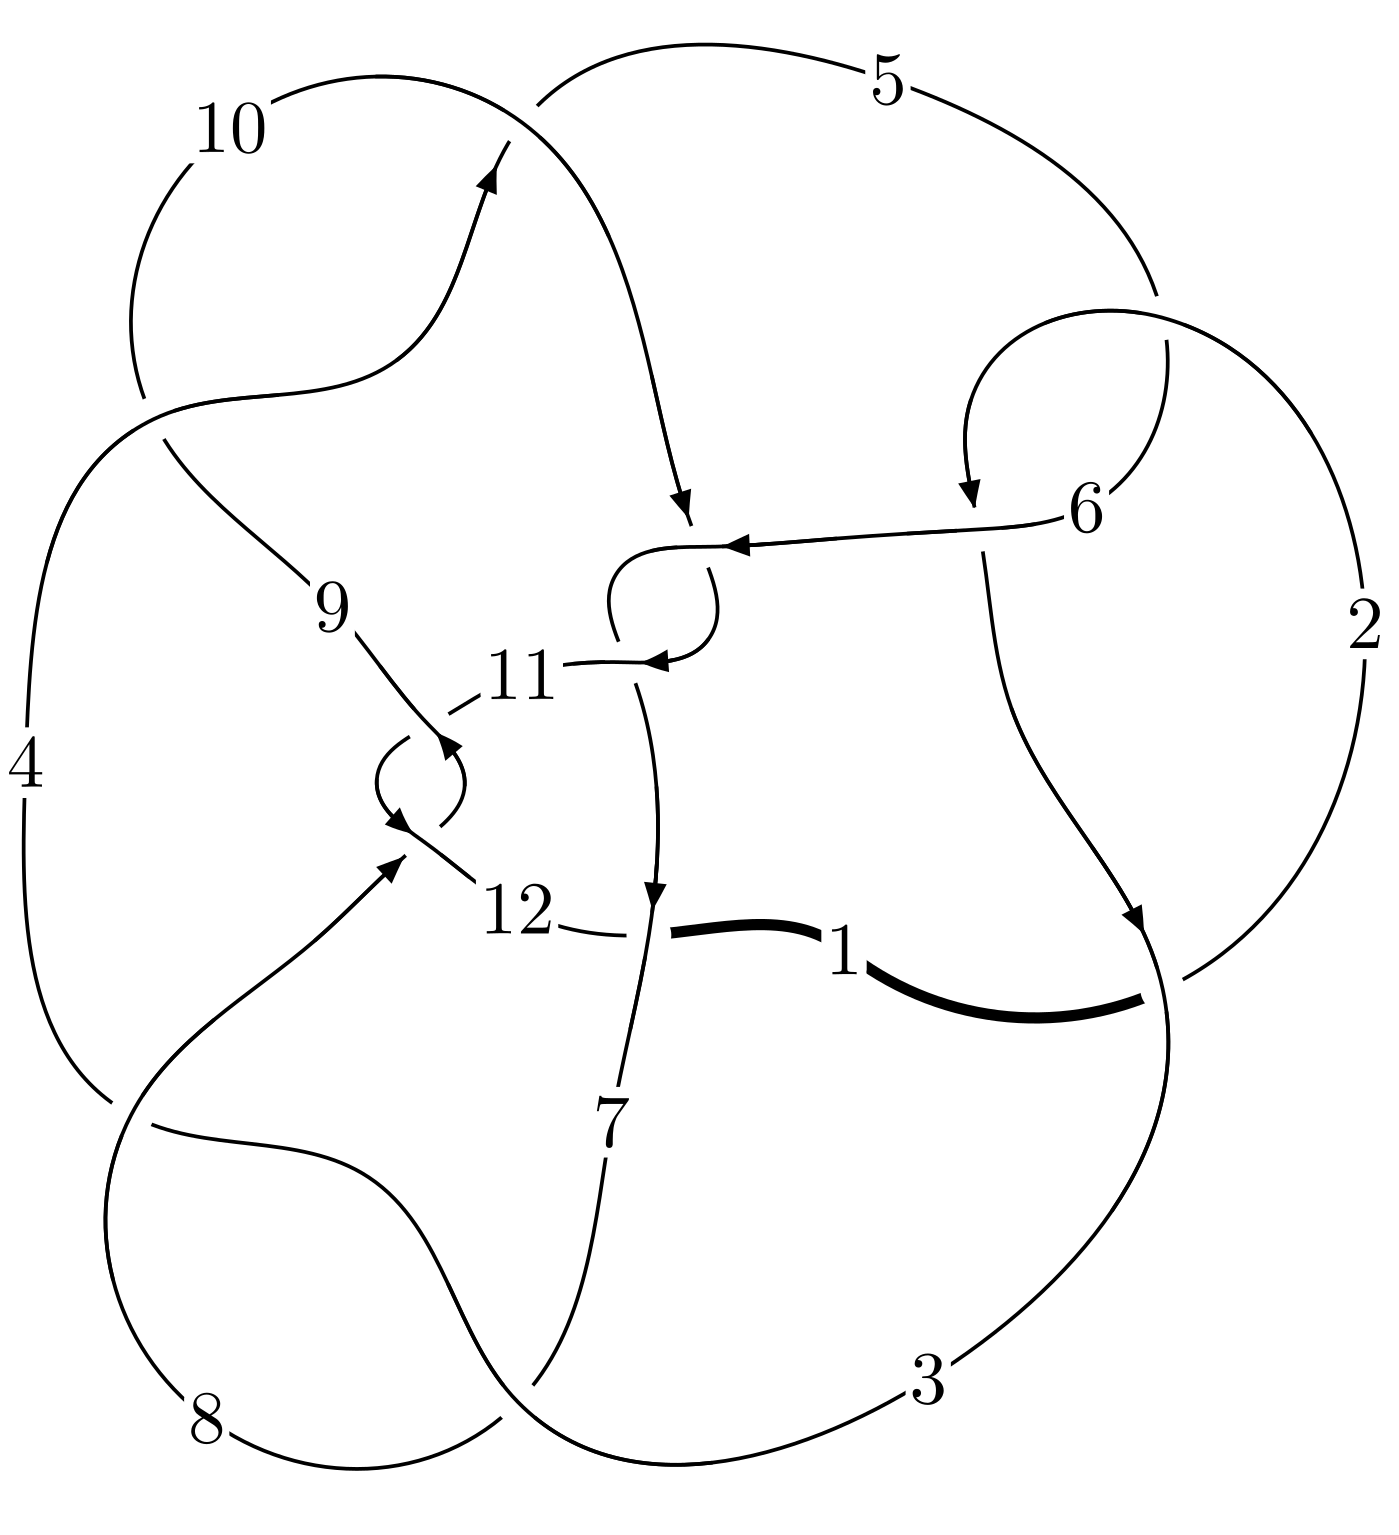
\includegraphics[width=112pt]{../../../GIT/diagram.site/Diagrams/png/2463_12n_0374.png}\\
\ \ \ A knot diagram\footnotemark}&
\allowdisplaybreaks
\textbf{Linearized knot diagam} \\
\cline{2-2}
 &
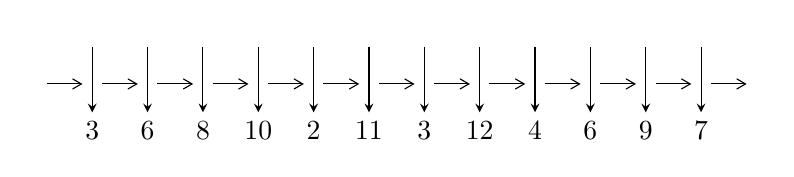
\begin{tikzpicture}[x=20pt, y=17pt]
	% nodes
	\node (C0) at (0, 0) {};
	\node (C1) at (1, 0) {};
	\node (C1U) at (1, +1) {};
	\node (C1D) at (1, -1) {3};

	\node (C2) at (2, 0) {};
	\node (C2U) at (2, +1) {};
	\node (C2D) at (2, -1) {6};

	\node (C3) at (3, 0) {};
	\node (C3U) at (3, +1) {};
	\node (C3D) at (3, -1) {8};

	\node (C4) at (4, 0) {};
	\node (C4U) at (4, +1) {};
	\node (C4D) at (4, -1) {10};

	\node (C5) at (5, 0) {};
	\node (C5U) at (5, +1) {};
	\node (C5D) at (5, -1) {2};

	\node (C6) at (6, 0) {};
	\node (C6U) at (6, +1) {};
	\node (C6D) at (6, -1) {11};

	\node (C7) at (7, 0) {};
	\node (C7U) at (7, +1) {};
	\node (C7D) at (7, -1) {3};

	\node (C8) at (8, 0) {};
	\node (C8U) at (8, +1) {};
	\node (C8D) at (8, -1) {12};

	\node (C9) at (9, 0) {};
	\node (C9U) at (9, +1) {};
	\node (C9D) at (9, -1) {4};

	\node (C10) at (10, 0) {};
	\node (C10U) at (10, +1) {};
	\node (C10D) at (10, -1) {6};

	\node (C11) at (11, 0) {};
	\node (C11U) at (11, +1) {};
	\node (C11D) at (11, -1) {9};

	\node (C12) at (12, 0) {};
	\node (C12U) at (12, +1) {};
	\node (C12D) at (12, -1) {7};
	\node (C13) at (13, 0) {};

	% arrows
	\draw[->,>={angle 60}]
	(C0) edge (C1) (C1) edge (C2) (C2) edge (C3) (C3) edge (C4) (C4) edge (C5) (C5) edge (C6) (C6) edge (C7) (C7) edge (C8) (C8) edge (C9) (C9) edge (C10) (C10) edge (C11) (C11) edge (C12) (C12) edge (C13) ;	\draw[->,>=stealth]
	(C1U) edge (C1D) (C2U) edge (C2D) (C3U) edge (C3D) (C4U) edge (C4D) (C5U) edge (C5D) (C6U) edge (C6D) (C7U) edge (C7D) (C8U) edge (C8D) (C9U) edge (C9D) (C10U) edge (C10D) (C11U) edge (C11D) (C12U) edge (C12D) ;
	\end{tikzpicture} \\
\hhline{~~} \\& 
\textbf{Solving Sequence} \\ \cline{2-2} 
 &
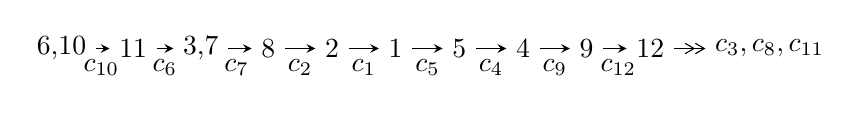
\begin{tikzpicture}[x=23pt, y=7pt]
	% node
	\node (A0) at (-1/8, 0) {6,10};
	\node (A1) at (1, 0) {11};
	\node (A2) at (33/16, 0) {3,7};
	\node (A3) at (25/8, 0) {8};
	\node (A4) at (33/8, 0) {2};
	\node (A5) at (41/8, 0) {1};
	\node (A6) at (49/8, 0) {5};
	\node (A7) at (57/8, 0) {4};
	\node (A8) at (65/8, 0) {9};
	\node (A9) at (73/8, 0) {12};
	\node (C1) at (1/2, -1) {$c_{10}$};
	\node (C2) at (3/2, -1) {$c_{6}$};
	\node (C3) at (21/8, -1) {$c_{7}$};
	\node (C4) at (29/8, -1) {$c_{2}$};
	\node (C5) at (37/8, -1) {$c_{1}$};
	\node (C6) at (45/8, -1) {$c_{5}$};
	\node (C7) at (53/8, -1) {$c_{4}$};
	\node (C8) at (61/8, -1) {$c_{9}$};
	\node (C9) at (69/8, -1) {$c_{12}$};
	\node (A10) at (11, 0) {$c_{3},c_{8},c_{11}$};

	% edge
	\draw[->,>=stealth]	
	(A0) edge (A1) (A1) edge (A2) (A2) edge (A3) (A3) edge (A4) (A4) edge (A5) (A5) edge (A6) (A6) edge (A7) (A7) edge (A8) (A8) edge (A9) ;
	\draw[->>,>={angle 60}]	
	(A9) edge (A10);
\end{tikzpicture} \\ 

\end{tabular} \\

\footnotetext{
The image of knot diagram is generated by the software ``\textbf{Draw programme}" developed by Andrew Bartholomew(\url{http://www.layer8.co.uk/maths/draw/index.htm\#Running-draw}), where we modified some parts for our purpose(\url{https://github.com/CATsTAILs/LinksPainter}).
}\phantom \\ \newline 
\centering \textbf{Ideals for irreducible components\footnotemark of $X_{\text{par}}$} 
 
\begin{align*}
I^u_{1}&=\langle 
-301149306547334 u^{15}-405785743495567 u^{14}+\cdots+5460935417391053 b-2324129620964575,\\
\phantom{I^u_{1}}&\phantom{= \langle  }2521976827730410 u^{15}+4134029936992622 u^{14}+\cdots+5460935417391053 a-8351550389039156,\\
\phantom{I^u_{1}}&\phantom{= \langle  }u^{16}+2 u^{15}+\cdots+u-1\rangle \\
I^u_{2}&=\langle 
u^9+u^8-2 u^7+2 u^6+3 u^5-6 u^4+2 u^2+b-2 u-1,\\
\phantom{I^u_{2}}&\phantom{= \langle  }u^{10}-4 u^8+2 u^7+4 u^6-6 u^5+u^4+4 u^3- u^2+a- u+1,\\
\phantom{I^u_{2}}&\phantom{= \langle  }u^{11}+u^{10}-3 u^9+5 u^7-4 u^6-4 u^5+4 u^4+u^3-3 u^2+1\rangle \\
\\
\end{align*}
\raggedright * 2 irreducible components of $\dim_{\mathbb{C}}=0$, with total 27 representations.\\
\footnotetext{All coefficients of polynomials are rational numbers. But the coefficients are sometimes approximated in decimal forms when there is not enough margin.}
\newpage
\renewcommand{\arraystretch}{1}
\centering \section*{I. $I^u_{1}= \langle -3.01\times10^{14} u^{15}-4.06\times10^{14} u^{14}+\cdots+5.46\times10^{15} b-2.32\times10^{15},\;2.52\times10^{15} u^{15}+4.13\times10^{15} u^{14}+\cdots+5.46\times10^{15} a-8.35\times10^{15},\;u^{16}+2 u^{15}+\cdots+u-1 \rangle$}
\flushleft \textbf{(i) Arc colorings}\\
\begin{tabular}{m{7pt} m{180pt} m{7pt} m{180pt} }
\flushright $a_{6}=$&$\begin{pmatrix}0\\u\end{pmatrix}$ \\
\flushright $a_{10}=$&$\begin{pmatrix}1\\0\end{pmatrix}$ \\
\flushright $a_{11}=$&$\begin{pmatrix}1\\u^2\end{pmatrix}$ \\
\flushright $a_{3}=$&$\begin{pmatrix}-0.461821 u^{15}-0.757019 u^{14}+\cdots+1.13267 u+1.52933\\0.0551461 u^{15}+0.0743070 u^{14}+\cdots-1.30799 u+0.425592\end{pmatrix}$ \\
\flushright $a_{7}=$&$\begin{pmatrix}- u\\- u^3+u\end{pmatrix}$ \\
\flushright $a_{8}=$&$\begin{pmatrix}-1.16646 u^{15}-2.14400 u^{14}+\cdots-0.648553 u+1.23228\\0.142447 u^{15}+0.241985 u^{14}+\cdots-2.03492 u+0.447884\end{pmatrix}$ \\
\flushright $a_{2}=$&$\begin{pmatrix}-0.461821 u^{15}-0.757019 u^{14}+\cdots+1.13267 u+1.52933\\0.0215283 u^{15}+0.0644709 u^{14}+\cdots-0.679549 u+0.258968\end{pmatrix}$ \\
\flushright $a_{1}=$&$\begin{pmatrix}1.49486 u^{15}+2.51422 u^{14}+\cdots-4.17011 u-0.263898\\-0.226698 u^{15}-0.0915071 u^{14}+\cdots+4.12577 u-0.807954\end{pmatrix}$ \\
\flushright $a_{5}=$&$\begin{pmatrix}1.28737 u^{15}+2.32151 u^{14}+\cdots-1.70682 u-1.04336\\-0.120918 u^{15}-0.177515 u^{14}+\cdots+2.35537 u-0.188916\end{pmatrix}$ \\
\flushright $a_{4}=$&$\begin{pmatrix}1.16646 u^{15}+2.14400 u^{14}+\cdots+0.648553 u-1.23228\\-0.120918 u^{15}-0.177515 u^{14}+\cdots+2.35537 u-0.188916\end{pmatrix}$ \\
\flushright $a_{9}=$&$\begin{pmatrix}0.802633 u^{15}+1.98845 u^{14}+\cdots+8.96383 u-3.11463\\-0.352889 u^{15}-0.635726 u^{14}+\cdots+0.487447 u+0.504102\end{pmatrix}$ \\
\flushright $a_{12}=$&$\begin{pmatrix}1.38603 u^{15}+2.45156 u^{14}+\cdots-2.59193 u-0.500660\\-0.149090 u^{15}-0.0711014 u^{14}+\cdots+2.28378 u-0.416208\end{pmatrix}$\\&\end{tabular}
\flushleft \textbf{(ii) Obstruction class $= -1$}\\~\\
\flushleft \textbf{(iii) Cusp Shapes $= -\frac{9739656845787569}{5460935417391053} u^{15}-\frac{17595322506035493}{5460935417391053} u^{14}+\cdots+\frac{16486080638841760}{5460935417391053} u-\frac{93508315704564998}{5460935417391053}$}\\~\\
\newpage\renewcommand{\arraystretch}{1}
\flushleft \textbf{(iv) u-Polynomials at the component}\newline \\
\begin{tabular}{m{50pt}|m{274pt}}
Crossings & \hspace{64pt}u-Polynomials at each crossing \\
\hline $$\begin{aligned}c_{1}\end{aligned}$$&$\begin{aligned}
&u^{16}-22 u^{15}+\cdots+28 u+1
\end{aligned}$\\
\hline $$\begin{aligned}c_{2},c_{5}\end{aligned}$$&$\begin{aligned}
&u^{16}+4 u^{15}+\cdots-2 u-1
\end{aligned}$\\
\hline $$\begin{aligned}c_{3},c_{7}\end{aligned}$$&$\begin{aligned}
&u^{16}-14 u^{15}+\cdots+152 u^2-32
\end{aligned}$\\
\hline $$\begin{aligned}c_{4},c_{9}\end{aligned}$$&$\begin{aligned}
&u^{16}+u^{15}+\cdots-184 u-85
\end{aligned}$\\
\hline $$\begin{aligned}c_{6},c_{10}\end{aligned}$$&$\begin{aligned}
&u^{16}-2 u^{15}+\cdots- u-1
\end{aligned}$\\
\hline $$\begin{aligned}c_{8},c_{11}\end{aligned}$$&$\begin{aligned}
&u^{16}-2 u^{15}+\cdots+2 u+1
\end{aligned}$\\
\hline $$\begin{aligned}c_{12}\end{aligned}$$&$\begin{aligned}
&u^{16}+8 u^{15}+\cdots-17328 u-2417
\end{aligned}$\\
\hline
\end{tabular}\\~\\
\newpage\renewcommand{\arraystretch}{1}
\flushleft \textbf{(v) Riley Polynomials at the component}\newline \\
\begin{tabular}{m{50pt}|m{274pt}}
Crossings & \hspace{64pt}Riley Polynomials at each crossing \\
\hline $$\begin{aligned}c_{1}\end{aligned}$$&$\begin{aligned}
&y^{16}+14 y^{15}+\cdots-540 y+1
\end{aligned}$\\
\hline $$\begin{aligned}c_{2},c_{5}\end{aligned}$$&$\begin{aligned}
&y^{16}+22 y^{15}+\cdots-28 y+1
\end{aligned}$\\
\hline $$\begin{aligned}c_{3},c_{7}\end{aligned}$$&$\begin{aligned}
&y^{16}-14 y^{15}+\cdots-9728 y+1024
\end{aligned}$\\
\hline $$\begin{aligned}c_{4},c_{9}\end{aligned}$$&$\begin{aligned}
&y^{16}+15 y^{15}+\cdots-36576 y+7225
\end{aligned}$\\
\hline $$\begin{aligned}c_{6},c_{10}\end{aligned}$$&$\begin{aligned}
&y^{16}+20 y^{15}+\cdots-9 y+1
\end{aligned}$\\
\hline $$\begin{aligned}c_{8},c_{11}\end{aligned}$$&$\begin{aligned}
&y^{16}+10 y^{15}+\cdots-14 y+1
\end{aligned}$\\
\hline $$\begin{aligned}c_{12}\end{aligned}$$&$\begin{aligned}
&y^{16}+38 y^{15}+\cdots-113705856 y+5841889
\end{aligned}$\\
\hline
\end{tabular}\\~\\
\newpage\flushleft \textbf{(vi) Complex Volumes and Cusp Shapes}
$$\begin{array}{c|c|c}  
\text{Solutions to }I^u_{1}& \I (\text{vol} + \sqrt{-1}CS) & \text{Cusp shape}\\
 \hline 
\begin{aligned}
u &= \phantom{-}0.709961 + 0.302018 I \\
a &= \phantom{-}0.067289 - 0.371265 I \\
b &= -1.56748 + 0.56103 I\end{aligned}
 & -2.10600 - 5.42693 I & -16.6708 + 2.3025 I \\ \hline\begin{aligned}
u &= \phantom{-}0.709961 - 0.302018 I \\
a &= \phantom{-}0.067289 + 0.371265 I \\
b &= -1.56748 - 0.56103 I\end{aligned}
 & -2.10600 + 5.42693 I & -16.6708 - 2.3025 I \\ \hline\begin{aligned}
u &= -0.624053 + 0.414470 I \\
a &= \phantom{-}0.036931 + 0.619361 I \\
b &= -0.268149 + 0.147042 I\end{aligned}
 & \phantom{-}2.12989 + 2.00985 I & -8.08247 - 3.69887 I \\ \hline\begin{aligned}
u &= -0.624053 - 0.414470 I \\
a &= \phantom{-}0.036931 - 0.619361 I \\
b &= -0.268149 - 0.147042 I\end{aligned}
 & \phantom{-}2.12989 - 2.00985 I & -8.08247 + 3.69887 I \\ \hline\begin{aligned}
u &= -0.603403\phantom{ +0.000000I} \\
a &= \phantom{-}0.346440\phantom{ +0.000000I} \\
b &= \phantom{-}1.97720\phantom{ +0.000000I}\end{aligned}
 & -5.59033\phantom{ +0.000000I} & -13.4830\phantom{ +0.000000I} \\ \hline\begin{aligned}
u &= \phantom{-}0.365789 + 0.462196 I \\
a &= \phantom{-}0.36041 - 1.55398 I \\
b &= \phantom{-}0.667180 + 0.526239 I\end{aligned}
 & -0.228166 + 0.909617 I & -12.89785 - 1.13498 I \\ \hline\begin{aligned}
u &= \phantom{-}0.365789 - 0.462196 I \\
a &= \phantom{-}0.36041 + 1.55398 I \\
b &= \phantom{-}0.667180 - 0.526239 I\end{aligned}
 & -0.228166 - 0.909617 I & -12.89785 + 1.13498 I \\ \hline\begin{aligned}
u &= -0.222804 + 0.369878 I \\
a &= \phantom{-}1.57769 + 3.86659 I \\
b &= \phantom{-}0.82840 - 1.19204 I\end{aligned}
 & -8.61028 - 1.60803 I & -19.3772 + 7.1837 I \\ \hline\begin{aligned}
u &= -0.222804 - 0.369878 I \\
a &= \phantom{-}1.57769 - 3.86659 I \\
b &= \phantom{-}0.82840 + 1.19204 I\end{aligned}
 & -8.61028 + 1.60803 I & -19.3772 - 7.1837 I \\ \hline\begin{aligned}
u &= \phantom{-}0.325252\phantom{ +0.000000I} \\
a &= \phantom{-}0.778005\phantom{ +0.000000I} \\
b &= \phantom{-}0.326406\phantom{ +0.000000I}\end{aligned}
 & -0.534698\phantom{ +0.000000I} & -18.5610\phantom{ +0.000000I}\\
 \hline 
 \end{array}$$\newpage$$\begin{array}{c|c|c}  
\text{Solutions to }I^u_{1}& \I (\text{vol} + \sqrt{-1}CS) & \text{Cusp shape}\\
 \hline 
\begin{aligned}
u &= \phantom{-}1.14699 + 2.11502 I \\
a &= \phantom{-}1.050490 + 0.062469 I \\
b &= -5.41647 + 5.13168 I\end{aligned}
 & \phantom{-}5.95217 - 5.11511 I & -14.9917 + 2.0744 I \\ \hline\begin{aligned}
u &= \phantom{-}1.14699 - 2.11502 I \\
a &= \phantom{-}1.050490 - 0.062469 I \\
b &= -5.41647 - 5.13168 I\end{aligned}
 & \phantom{-}5.95217 + 5.11511 I & -14.9917 - 2.0744 I \\ \hline\begin{aligned}
u &= -0.86624 + 2.26332 I \\
a &= -1.018240 + 0.164220 I \\
b &= \phantom{-}6.83232 + 3.44115 I\end{aligned}
 & \phantom{-}10.23600 + 0.21137 I & -11.36887 + 0.55661 I \\ \hline\begin{aligned}
u &= -0.86624 - 2.26332 I \\
a &= -1.018240 - 0.164220 I \\
b &= \phantom{-}6.83232 - 3.44115 I\end{aligned}
 & \phantom{-}10.23600 - 0.21137 I & -11.36887 - 0.55661 I \\ \hline\begin{aligned}
u &= -1.37057 + 2.24654 I \\
a &= -1.136800 + 0.049742 I \\
b &= \phantom{-}5.77240 + 7.05674 I\end{aligned}
 & \phantom{-}9.6708 + 10.3555 I & -12.00000 - 4.83541 I \\ \hline\begin{aligned}
u &= -1.37057 - 2.24654 I \\
a &= -1.136800 - 0.049742 I \\
b &= \phantom{-}5.77240 - 7.05674 I\end{aligned}
 & \phantom{-}9.6708 - 10.3555 I & -12.00000 + 4.83541 I\\
 \hline 
 \end{array}$$\newpage\newpage\renewcommand{\arraystretch}{1}
\centering \section*{II. $I^u_{2}= \langle u^9+u^8+\cdots+b-1,\;u^{10}-4 u^8+\cdots+a+1,\;u^{11}+u^{10}+\cdots-3 u^2+1 \rangle$}
\flushleft \textbf{(i) Arc colorings}\\
\begin{tabular}{m{7pt} m{180pt} m{7pt} m{180pt} }
\flushright $a_{6}=$&$\begin{pmatrix}0\\u\end{pmatrix}$ \\
\flushright $a_{10}=$&$\begin{pmatrix}1\\0\end{pmatrix}$ \\
\flushright $a_{11}=$&$\begin{pmatrix}1\\u^2\end{pmatrix}$ \\
\flushright $a_{3}=$&$\begin{pmatrix}- u^{10}+4 u^8-2 u^7-4 u^6+6 u^5- u^4-4 u^3+u^2+u-1\\- u^9- u^8+2 u^7-2 u^6-3 u^5+6 u^4-2 u^2+2 u+1\end{pmatrix}$ \\
\flushright $a_{7}=$&$\begin{pmatrix}- u\\- u^3+u\end{pmatrix}$ \\
\flushright $a_{8}=$&$\begin{pmatrix}- u^9- u^8+3 u^7-5 u^5+3 u^4+3 u^3-2 u^2- u+1\\2 u^9+2 u^8-5 u^7+6 u^5-6 u^4-3 u^3+2 u^2- u-1\end{pmatrix}$ \\
\flushright $a_{2}=$&$\begin{pmatrix}- u^{10}+4 u^8-2 u^7-4 u^6+6 u^5- u^4-4 u^3+u^2+u-1\\-2 u^9-2 u^8+5 u^7- u^6-7 u^5+8 u^4+3 u^3-4 u^2+u+2\end{pmatrix}$ \\
\flushright $a_{1}=$&$\begin{pmatrix}u^9+u^8-3 u^7- u^6+4 u^5- u^4-2 u^3\\-2 u^9-3 u^8+4 u^7+3 u^6-4 u^5+2 u^4+u^3+u^2+u\end{pmatrix}$ \\
\flushright $a_{5}=$&$\begin{pmatrix}u^9+u^8-3 u^7- u^6+4 u^5- u^4-3 u^3+2 u\\u^6+u^5-2 u^4+2 u^2- u-1\end{pmatrix}$ \\
\flushright $a_{4}=$&$\begin{pmatrix}u^9+u^8-3 u^7+5 u^5-3 u^4-3 u^3+2 u^2+u-1\\u^6+u^5-2 u^4+2 u^2- u-1\end{pmatrix}$ \\
\flushright $a_{9}=$&$\begin{pmatrix}u^8+u^7-3 u^6-2 u^5+3 u^4-3 u^2+2\\u^{10}+u^9-3 u^8- u^7+4 u^6-2 u^5-3 u^4+2 u^3- u\end{pmatrix}$ \\
\flushright $a_{12}=$&$\begin{pmatrix}u^4-2 u^2+1\\- u^9- u^8+2 u^7-2 u^5+2 u^4+u^2+u\end{pmatrix}$\\&\end{tabular}
\flushleft \textbf{(ii) Obstruction class $= 1$}\\~\\
\flushleft \textbf{(iii) Cusp Shapes $= 4 u^{10}+10 u^9-2 u^8-14 u^7+9 u^6+15 u^5-26 u^4-23 u^3+22 u^2-2 u-29$}\\~\\
\newpage\renewcommand{\arraystretch}{1}
\flushleft \textbf{(iv) u-Polynomials at the component}\newline \\
\begin{tabular}{m{50pt}|m{274pt}}
Crossings & \hspace{64pt}u-Polynomials at each crossing \\
\hline $$\begin{aligned}c_{1}\end{aligned}$$&$\begin{aligned}
&u^{11}-9 u^{10}+\cdots+5 u-1
\end{aligned}$\\
\hline $$\begin{aligned}c_{2}\end{aligned}$$&$\begin{aligned}
&u^{11}+3 u^{10}-6 u^8-2 u^7+2 u^6+3 u^5+4 u^4+2 u^3-2 u^2-3 u-1
\end{aligned}$\\
\hline $$\begin{aligned}c_{3}\end{aligned}$$&$\begin{aligned}
&u^{11}+2 u^{10}+\cdots-5 u+1
\end{aligned}$\\
\hline $$\begin{aligned}c_{4}\end{aligned}$$&$\begin{aligned}
&u^{11}-4 u^9-6 u^8+10 u^7+23 u^6-10 u^5-23 u^4-2 u^3+16 u^2-3 u-1
\end{aligned}$\\
\hline $$\begin{aligned}c_{5}\end{aligned}$$&$\begin{aligned}
&u^{11}-3 u^{10}+6 u^8-2 u^7-2 u^6+3 u^5-4 u^4+2 u^3+2 u^2-3 u+1
\end{aligned}$\\
\hline $$\begin{aligned}c_{6}\end{aligned}$$&$\begin{aligned}
&u^{11}- u^{10}-3 u^9+5 u^7+4 u^6-4 u^5-4 u^4+u^3+3 u^2-1
\end{aligned}$\\
\hline $$\begin{aligned}c_{7}\end{aligned}$$&$\begin{aligned}
&u^{11}-2 u^{10}+\cdots-5 u-1
\end{aligned}$\\
\hline $$\begin{aligned}c_{8}\end{aligned}$$&$\begin{aligned}
&u^{11}-3 u^{10}+\cdots- u+1
\end{aligned}$\\
\hline $$\begin{aligned}c_{9}\end{aligned}$$&$\begin{aligned}
&u^{11}-4 u^9+6 u^8+10 u^7-23 u^6-10 u^5+23 u^4-2 u^3-16 u^2-3 u+1
\end{aligned}$\\
\hline $$\begin{aligned}c_{10}\end{aligned}$$&$\begin{aligned}
&u^{11}+u^{10}-3 u^9+5 u^7-4 u^6-4 u^5+4 u^4+u^3-3 u^2+1
\end{aligned}$\\
\hline $$\begin{aligned}c_{11}\end{aligned}$$&$\begin{aligned}
&u^{11}+3 u^{10}+\cdots- u-1
\end{aligned}$\\
\hline $$\begin{aligned}c_{12}\end{aligned}$$&$\begin{aligned}
&u^{11}-7 u^{10}+\cdots-85 u+29
\end{aligned}$\\
\hline
\end{tabular}\\~\\
\newpage\renewcommand{\arraystretch}{1}
\flushleft \textbf{(v) Riley Polynomials at the component}\newline \\
\begin{tabular}{m{50pt}|m{274pt}}
Crossings & \hspace{64pt}Riley Polynomials at each crossing \\
\hline $$\begin{aligned}c_{1}\end{aligned}$$&$\begin{aligned}
&y^{11}-17 y^{10}+\cdots+9 y-1
\end{aligned}$\\
\hline $$\begin{aligned}c_{2},c_{5}\end{aligned}$$&$\begin{aligned}
&y^{11}-9 y^{10}+\cdots+5 y-1
\end{aligned}$\\
\hline $$\begin{aligned}c_{3},c_{7}\end{aligned}$$&$\begin{aligned}
&y^{11}-14 y^{10}+\cdots+21 y-1
\end{aligned}$\\
\hline $$\begin{aligned}c_{4},c_{9}\end{aligned}$$&$\begin{aligned}
&y^{11}-8 y^{10}+\cdots+41 y-1
\end{aligned}$\\
\hline $$\begin{aligned}c_{6},c_{10}\end{aligned}$$&$\begin{aligned}
&y^{11}-7 y^{10}+\cdots+6 y-1
\end{aligned}$\\
\hline $$\begin{aligned}c_{8},c_{11}\end{aligned}$$&$\begin{aligned}
&y^{11}+7 y^{10}+\cdots+3 y-1
\end{aligned}$\\
\hline $$\begin{aligned}c_{12}\end{aligned}$$&$\begin{aligned}
&y^{11}-21 y^{10}+\cdots+10821 y-841
\end{aligned}$\\
\hline
\end{tabular}\\~\\
\newpage\flushleft \textbf{(vi) Complex Volumes and Cusp Shapes}
$$\begin{array}{c|c|c}  
\text{Solutions to }I^u_{2}& \I (\text{vol} + \sqrt{-1}CS) & \text{Cusp shape}\\
 \hline 
\begin{aligned}
u &= \phantom{-}0.636123 + 0.670136 I \\
a &= \phantom{-}1.114440 - 0.543604 I \\
b &= -0.780678 + 0.831560 I\end{aligned}
 & \phantom{-}1.01561 - 3.68794 I & -9.46045 + 4.33638 I \\ \hline\begin{aligned}
u &= \phantom{-}0.636123 - 0.670136 I \\
a &= \phantom{-}1.114440 + 0.543604 I \\
b &= -0.780678 - 0.831560 I\end{aligned}
 & \phantom{-}1.01561 + 3.68794 I & -9.46045 - 4.33638 I \\ \hline\begin{aligned}
u &= \phantom{-}0.579598 + 0.909451 I \\
a &= -0.53978 + 1.76442 I \\
b &= -1.78870 - 1.78170 I\end{aligned}
 & -8.26462 + 1.07707 I & -11.60559 + 3.04504 I \\ \hline\begin{aligned}
u &= \phantom{-}0.579598 - 0.909451 I \\
a &= -0.53978 - 1.76442 I \\
b &= -1.78870 + 1.78170 I\end{aligned}
 & -8.26462 - 1.07707 I & -11.60559 - 3.04504 I \\ \hline\begin{aligned}
u &= \phantom{-}1.16659\phantom{ +0.000000I} \\
a &= -0.621653\phantom{ +0.000000I} \\
b &= -1.35028\phantom{ +0.000000I}\end{aligned}
 & -8.04334\phantom{ +0.000000I} & -20.3040\phantom{ +0.000000I} \\ \hline\begin{aligned}
u &= -0.693012 + 0.407011 I \\
a &= \phantom{-}0.911623 - 0.220211 I \\
b &= -2.23098 - 0.93364 I\end{aligned}
 & -1.97384 + 6.11246 I & -15.4629 - 13.1582 I \\ \hline\begin{aligned}
u &= -0.693012 - 0.407011 I \\
a &= \phantom{-}0.911623 + 0.220211 I \\
b &= -2.23098 + 0.93364 I\end{aligned}
 & -1.97384 - 6.11246 I & -15.4629 + 13.1582 I \\ \hline\begin{aligned}
u &= -0.733849\phantom{ +0.000000I} \\
a &= -1.28586\phantom{ +0.000000I} \\
b &= \phantom{-}0.269849\phantom{ +0.000000I}\end{aligned}
 & -2.65454\phantom{ +0.000000I} & -14.9220\phantom{ +0.000000I} \\ \hline\begin{aligned}
u &= \phantom{-}0.710299\phantom{ +0.000000I} \\
a &= -0.858009\phantom{ +0.000000I} \\
b &= \phantom{-}2.21118\phantom{ +0.000000I}\end{aligned}
 & -6.08165\phantom{ +0.000000I} & -31.1290\phantom{ +0.000000I} \\ \hline\begin{aligned}
u &= -1.59423 + 0.15020 I \\
a &= -0.103519 + 0.553154 I \\
b &= \phantom{-}0.73498 + 1.21716 I\end{aligned}
 & -5.41647 - 2.99510 I & -12.79336 + 4.15050 I\\
 \hline 
 \end{array}$$\newpage$$\begin{array}{c|c|c}  
\text{Solutions to }I^u_{2}& \I (\text{vol} + \sqrt{-1}CS) & \text{Cusp shape}\\
 \hline 
\begin{aligned}
u &= -1.59423 - 0.15020 I \\
a &= -0.103519 - 0.553154 I \\
b &= \phantom{-}0.73498 - 1.21716 I\end{aligned}
 & -5.41647 + 2.99510 I & -12.79336 - 4.15050 I\\
 \hline 
 \end{array}$$\newpage
\newpage\renewcommand{\arraystretch}{1}
\centering \section*{ III. u-Polynomials}
\begin{tabular}{m{50pt}|m{274pt}}
Crossings & \hspace{64pt}u-Polynomials at each crossing \\
\hline $$\begin{aligned}c_{1}\end{aligned}$$&$\begin{aligned}
&(u^{11}-9 u^{10}+\cdots+5 u-1)(u^{16}-22 u^{15}+\cdots+28 u+1)
\end{aligned}$\\
\hline $$\begin{aligned}c_{2}\end{aligned}$$&$\begin{aligned}
&(u^{11}+3 u^{10}-6 u^8-2 u^7+2 u^6+3 u^5+4 u^4+2 u^3-2 u^2-3 u-1)\\
&\cdot(u^{16}+4 u^{15}+\cdots-2 u-1)
\end{aligned}$\\
\hline $$\begin{aligned}c_{3}\end{aligned}$$&$\begin{aligned}
&(u^{11}+2 u^{10}+\cdots-5 u+1)(u^{16}-14 u^{15}+\cdots+152 u^2-32)
\end{aligned}$\\
\hline $$\begin{aligned}c_{4}\end{aligned}$$&$\begin{aligned}
&(u^{11}-4 u^9-6 u^8+10 u^7+23 u^6-10 u^5-23 u^4-2 u^3+16 u^2-3 u-1)\\
&\cdot(u^{16}+u^{15}+\cdots-184 u-85)
\end{aligned}$\\
\hline $$\begin{aligned}c_{5}\end{aligned}$$&$\begin{aligned}
&(u^{11}-3 u^{10}+6 u^8-2 u^7-2 u^6+3 u^5-4 u^4+2 u^3+2 u^2-3 u+1)\\
&\cdot(u^{16}+4 u^{15}+\cdots-2 u-1)
\end{aligned}$\\
\hline $$\begin{aligned}c_{6}\end{aligned}$$&$\begin{aligned}
&(u^{11}- u^{10}-3 u^9+5 u^7+4 u^6-4 u^5-4 u^4+u^3+3 u^2-1)\\
&\cdot(u^{16}-2 u^{15}+\cdots- u-1)
\end{aligned}$\\
\hline $$\begin{aligned}c_{7}\end{aligned}$$&$\begin{aligned}
&(u^{11}-2 u^{10}+\cdots-5 u-1)(u^{16}-14 u^{15}+\cdots+152 u^2-32)
\end{aligned}$\\
\hline $$\begin{aligned}c_{8}\end{aligned}$$&$\begin{aligned}
&(u^{11}-3 u^{10}+\cdots- u+1)(u^{16}-2 u^{15}+\cdots+2 u+1)
\end{aligned}$\\
\hline $$\begin{aligned}c_{9}\end{aligned}$$&$\begin{aligned}
&(u^{11}-4 u^9+6 u^8+10 u^7-23 u^6-10 u^5+23 u^4-2 u^3-16 u^2-3 u+1)\\
&\cdot(u^{16}+u^{15}+\cdots-184 u-85)
\end{aligned}$\\
\hline $$\begin{aligned}c_{10}\end{aligned}$$&$\begin{aligned}
&(u^{11}+u^{10}-3 u^9+5 u^7-4 u^6-4 u^5+4 u^4+u^3-3 u^2+1)\\
&\cdot(u^{16}-2 u^{15}+\cdots- u-1)
\end{aligned}$\\
\hline $$\begin{aligned}c_{11}\end{aligned}$$&$\begin{aligned}
&(u^{11}+3 u^{10}+\cdots- u-1)(u^{16}-2 u^{15}+\cdots+2 u+1)
\end{aligned}$\\
\hline $$\begin{aligned}c_{12}\end{aligned}$$&$\begin{aligned}
&(u^{11}-7 u^{10}+\cdots-85 u+29)(u^{16}+8 u^{15}+\cdots-17328 u-2417)
\end{aligned}$\\
\hline
\end{tabular}\newpage\renewcommand{\arraystretch}{1}
\centering \section*{ IV. Riley Polynomials}
\begin{tabular}{m{50pt}|m{274pt}}
Crossings & \hspace{64pt}Riley Polynomials at each crossing \\
\hline $$\begin{aligned}c_{1}\end{aligned}$$&$\begin{aligned}
&(y^{11}-17 y^{10}+\cdots+9 y-1)(y^{16}+14 y^{15}+\cdots-540 y+1)
\end{aligned}$\\
\hline $$\begin{aligned}c_{2},c_{5}\end{aligned}$$&$\begin{aligned}
&(y^{11}-9 y^{10}+\cdots+5 y-1)(y^{16}+22 y^{15}+\cdots-28 y+1)
\end{aligned}$\\
\hline $$\begin{aligned}c_{3},c_{7}\end{aligned}$$&$\begin{aligned}
&(y^{11}-14 y^{10}+\cdots+21 y-1)(y^{16}-14 y^{15}+\cdots-9728 y+1024)
\end{aligned}$\\
\hline $$\begin{aligned}c_{4},c_{9}\end{aligned}$$&$\begin{aligned}
&(y^{11}-8 y^{10}+\cdots+41 y-1)(y^{16}+15 y^{15}+\cdots-36576 y+7225)
\end{aligned}$\\
\hline $$\begin{aligned}c_{6},c_{10}\end{aligned}$$&$\begin{aligned}
&(y^{11}-7 y^{10}+\cdots+6 y-1)(y^{16}+20 y^{15}+\cdots-9 y+1)
\end{aligned}$\\
\hline $$\begin{aligned}c_{8},c_{11}\end{aligned}$$&$\begin{aligned}
&(y^{11}+7 y^{10}+\cdots+3 y-1)(y^{16}+10 y^{15}+\cdots-14 y+1)
\end{aligned}$\\
\hline $$\begin{aligned}c_{12}\end{aligned}$$&$\begin{aligned}
&(y^{11}-21 y^{10}+\cdots+10821 y-841)\\
&\cdot(y^{16}+38 y^{15}+\cdots-113705856 y+5841889)
\end{aligned}$\\
\hline
\end{tabular}
\vskip 2pc
\end{document}